\documentclass[hyphens]{beamer}

\usepackage[utf8]{inputenc}
\usepackage[ngerman]{babel}

\usepackage{array}
\usepackage{tabularx}
\newcolumntype{Z}{>{\centering\let\newline\\\arraybackslash\hspace{0pt}}p{0.65\textwidth}}

\usepackage{amssymb}
\usepackage{pifont}
\newcommand{\xmark}{\ding{55}}
\usepackage{svg}

\usetheme[progressbar=frametitle,block=fill]{metropolis}

\setbeamertemplate{section in toc}[sections numbered]
\setbeamertemplate{subsection in toc}[subsections numbered]
\setbeamertemplate{caption}{\raggedright\insertcaption\par}

\defbeamertemplate{subsubsection in toc}{subsubsections numbered}
{\leavevmode\leftskip=3em%
 \rlap{\hskip-3em\inserttocsectionnumber.\inserttocsubsectionnumber.\inserttocsubsubsectionnumber}%
 \inserttocsubsubsection\par}

\setbeamertemplate{subsubsection in toc}[subsubsections numbered]

\begin{document}
  \title[Gerät zur Schlaganfall-Rehabilitation]{Entwicklung eines Gamification-basierten Unterstützungs- und Motivationsgeräts zur Rehabilitation von Schlaganfall-Patienten \\ \small{- Kolloquium -}}
  \author[Lukas Rost]{Lukas Rost  \\ \and \emph{Fachbetreuer:} Johannes Süpke \\ \and \emph{Außenbetreuer:} Hannes Weichel (topdev GmbH)}
  \institute[ASGspez]{Spezialschulteil des staatlichen Gymnasiums "'Albert Schweitzer"' Erfurt}
  \date{20. März 2019}

 \begin{frame}
 \titlepage
 \end{frame}

  \begin{frame}
\begin{figure}
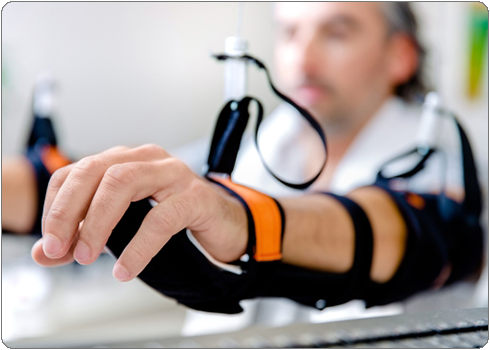
\includegraphics[scale=0.6]{../Themenverteidigung/pics/einleit1}
  \caption{Therapiegerät für Armlähmungen}
\end{figure}
 \end{frame}

 \begin{frame}
 \titlepage
 \end{frame}

 \begin{frame}{Gliederung}
 \tableofcontents
 \end{frame}

%TODO TODO TODO

 \section{Kritische Reflexion des Erreichten}
 \begin{frame}{Kritische Reflexion des Erreichten}
 \end{frame}

 \begin{frame}{Bildquellen}
 \begin{itemize}
 \item \small{\url{https://raw.githubusercontent.com/SeeedDocument/Grove-EMG_Detector/master/img/Emg_connect.jpg}}
 \item \small{\url{https://upload.wikimedia.org/wikipedia/commons/7/74/Kotlin-logo.svg}}
 \item \small{\url{https://upload.wikimedia.org/wikipedia/commons/1/17/OpenGL_ES_Nov14.svg}}
 \item \small{selbst erstellt}
 \end{itemize}
 \end{frame}

 \begin{frame}
 \titlepage
 \end{frame}

\end{document}
